\chapter{Implementation}

%The implementation should discuss any issues you encountered as you tried to implement your design. During the work, you might have found that elements of your design were unnecessary or overly complex; perhaps third-party libraries were available that simplified some of the functions that you intended to implement. If things were easier in some areas, then how did you adapt your project to take account of your findings?
%
%It is more likely that things were more complex than you first thought. In particular, were there any problems or difficulties that you found during implementation that you had to address? Did such problems simply delay you or were they more significant?
%
%You can conclude this section by reviewing the end of the implementation stage against the planned requirements. 

\section{Code Implementation \& Third-Party libraries}
As seen below the Website and Discord bots have been split up into two separate sections because during implementation I decided to make the systems separate. This helps with code maintainability, readability and allows the administrator who sets up this project to deploy the website and bot services on different containers or networks.

\subsection{Website Building}
To create and run the website I've used a set of different libraries to perform certain tasks. Firstly I've used the Apache2 \cite{apache2} web hosting framework to host the website along with the library libapache2-mod-auth-openidc to reroute all incoming traffic to OpenID Connect \cite{OpenID} for user authentication. On top of these I have used the linux tool certbot \cite{certbot} to create a Let's Encrypt certificate for the website to enable HTTPS. 

As discussed previously in this document in section \ref{sec1:Research} there were many libraries that were considered when deciding on the website framework. Django \cite{Django} was the framework of choice and it is open-source and free to use on personal projects ( \href{https://www.djangoproject.com/trademarks/\#:~:text=Django\%20is\%20an\%20Open\%20Source,the\%20use\%20of\%20a\%20trademark.}{Django Trademark License Agreement}). It is also very useful as it generates the majority of the code required to create and run a website so most of the code used will be picked up by the system for UAP. Apart from the general template I created a "Django Application" called login that contains the files and code which is used to run the website and it's respective services.

The website pages also use a third party library called bootstrap \cite{bootstrap} that is used to generate responsive mobile-first CSS on the website.

\subsection{Discord Bot}
AberLink uses the Python library Discord.py \cite{discord.py} to make calls to and from the Discord API and to interact with the database it uses the Python library Psycopg2 \cite{psycopg2}. Both of these pieces of software are open-source and free to use in personal projects.

\section{Unforeseen Issues}\label{sec3:unforeseen}
An issue that I encountered was with creating the custom user model in Django that would have been used to model the database. The documentation and videos I found online about implementing user models were rather cryptic and difficult to understand, however I eventually found a video explaining how to implement a good custom user model. Once this was completed I realised that Django isn't happy with modelling the primary key of a table using a char so I had to switch to using an int. This turned out to be a good idea as Aberystwyth university tends to recycle old emails so over the next 5 years there could be an issue where the database would try and create a new entry in the database with the same email.

\section{Review Against Planned Requirements}
Most of the planned requirements haven't changed during implementation however as discussed in the section above \ref{sec3:unforeseen} the database model has changed slightly and the updated diagram is included below.
\begin{figure}[H]
	\centering
	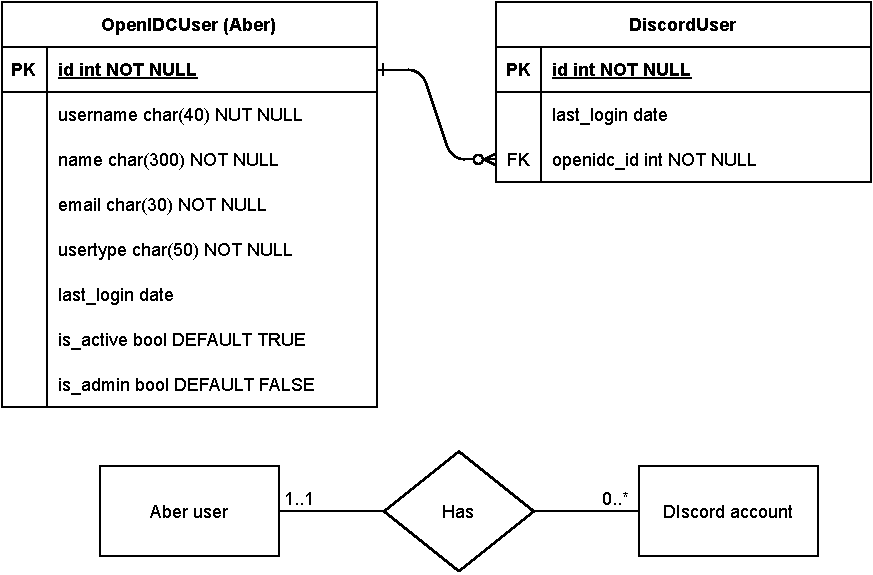
\includegraphics[width=0.8\linewidth]{Figures/database-er-1}
	\caption{Updated Entity relationship diagram for database}
	\label{fig:database-er-1}
\end{figure}

The planned requirements also included a section called \textbf{Interface for lecturers and students on website} has also only been partially fulfilled. I have completed the second part of this task which was to create admin pages to view the connected staff and students however the first part where users can view what servers they are in is missing. This was a design choice that I made because I realised that this would require that Discord servers are added to database and that they would have to be updated when any issues occurred. This was also bad because this list would have to be maintained and couldn't be automatically updated which would lead to it breaking down the line.

In the final section of the planned requirements \textbf{Further potential work} I have decided against integrating DemoHelper into AberLink as this would greatly increase it's complexity and make it much more difficult to maintain.